% Copyright (C) 2014-2015 Institut National de la Recherche Agronomique (INRA)
% License: Creative Commons Attribution-NonCommercial-ShareAlike 4.0 International
% Person: Timothée Flutre [cre,aut]

\documentclass[c]{beamer} % use [t] to top-justified body text by default
% \documentclass[c,handout]{beamer}
\usepackage{graphicx}
\usepackage{xcolor}
\definecolor{gray}{gray}{0.35}
\usepackage{hyperref}
\hypersetup{colorlinks, linkcolor=black, urlcolor=gray}
\usepackage{amsmath}
\usepackage{bm} % to have mathematical symbols in bold
\usepackage{multirow}
\usepackage{tikz}
\usepackage[francais]{babel}
\usepackage[utf8]{inputenc}

\graphicspath{{./figures/}}

% -----------------------------------------------------------------------------

\setbeamertemplate{navigation symbols}{}
\setbeamercolor{alerted text}{fg=purple}
\setbeamertemplate{caption}[numbered]
\setbeamerfont{caption}{size=\scriptsize}
\setbeameroption{hide notes}
% \setbeameroption{show notes}
\setbeamertemplate{note page}[plain]

\setbeamertemplate{footline}
{
  \leavevmode
  \hbox{
    \hspace*{-0.06cm}
    \begin{beamercolorbox}[wd=.2\paperwidth,ht=2.25ex,dp=1ex,center]{author in head/foot}
      \usebeamerfont{author in head/foot}\insertshortauthor \hspace*{1em} \insertshortinstitute
    \end{beamercolorbox}
    \begin{beamercolorbox}[wd=.50\paperwidth,ht=2.25ex,dp=1ex,center]{section in head/foot}
      \usebeamerfont{section in head/foot}\insertshorttitle
    \end{beamercolorbox}
    \begin{beamercolorbox}[wd=.27\paperwidth,ht=2.25ex,dp=1ex,right]{section in head/foot}%
      \usebeamerfont{section in head/foot}\insertshortdate{}\hspace*{2em}
      \insertframenumber{} / \inserttotalframenumber\hspace*{2ex}
    \end{beamercolorbox}
  }
  \vskip0pt
}

\AtBeginSection[]
{
  \begin{frame}
    \frametitle{Outline}
    \addtocounter{framenumber}{-1}
    \tableofcontents[currentsection]
  \end{frame}
}

% -----------------------------------------------------------------------------

\title[Reproducible research]{Caring about reproducibility in scientific research}
\author[T. Flutre]{Timoth\'{e}e Flutre}
\institute[INRA]{INRA, UMR AGAP}
\date{08/12/2014}

\begin{document}

\begin{frame}
  \titlepage
  
  \tiny
  \begin{center}
    Last updated: 16/06/2015
    
    \medskip
    
    License: \href{http://creativecommons.org/licenses/by-nc-sa/4.0/}{CC BY-NC-SA 4.0}
  \end{center}
\end{frame}                                                                                                                       
\begin{frame}
  \frametitle{Abstract}
  \tiny
  Sooner or later, any research effort implies some data collection in light of a scientific theory, which in turn implies some data analysis. In practice, we enter the raw data in a computer and use a program to fit a model. But soon enough we change the model, add a preprocessing step, collect more data, share our on-going work with a student in the nearby office or with a collaborator abroad, etc. And in a realistic research project, we do this again, and again, and again... Such a process is now often called "computational science". In this context, we usually want to keep track of what we do and, even better, what our student/collaborator do. We would also like to better understand what other teams did in their recently-published paper and, why not, apply their code on our data or even combine their data with ours.
  
  \medskip
  
  In this presentation, I will rapidly outline the current state of affairs about reproducibility in research and what it says for code and data. I will then present in some details the computational tools I am using, after years of trials and errors and inspirations from many people. In the end, everyone is welcome to bring his computer to try by himself on a minimal case study (many cables will be available for internet connection).
  
  \bigskip
  
  In these slides, terms in \textcolor{gray}{grey} correspond to HTML links: click on them ;)
\end{frame}

\begin{frame}
  \frametitle{Outline}
  \tableofcontents
\end{frame}

\section{Global context}

\begin{frame}
  \frametitle{Statistical Inference: the Big Picture (\href{http://dx.doi.org/10.1214/10-sts337}{Kass, 2011})}
  \only<1>{
    \begin{center}
      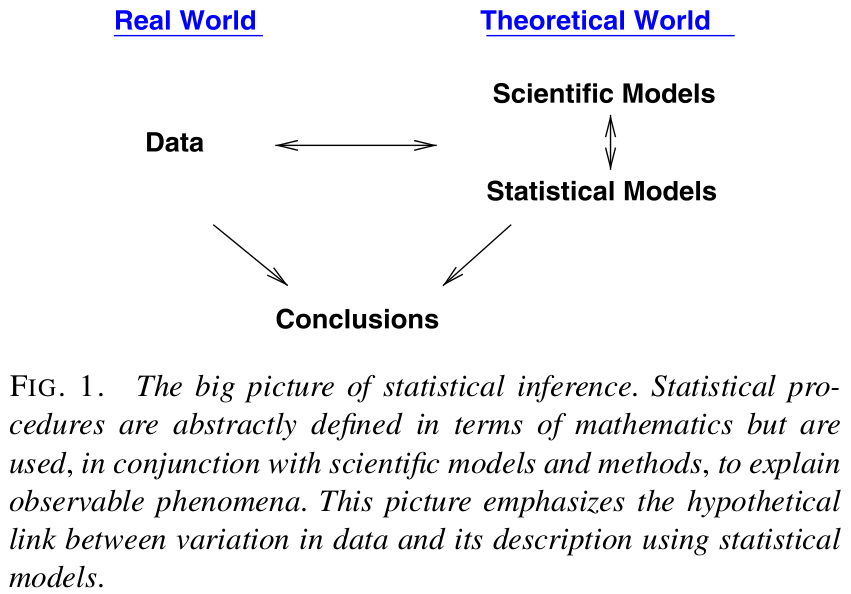
\includegraphics[width=0.8\textwidth,height=0.80\textheight,keepaspectratio=true]{kass_11_statistical-inference_fig1}%
    \end{center}
  }
  \only<2>{
    Standard conception:
    \bigskip
    \begin{center}
      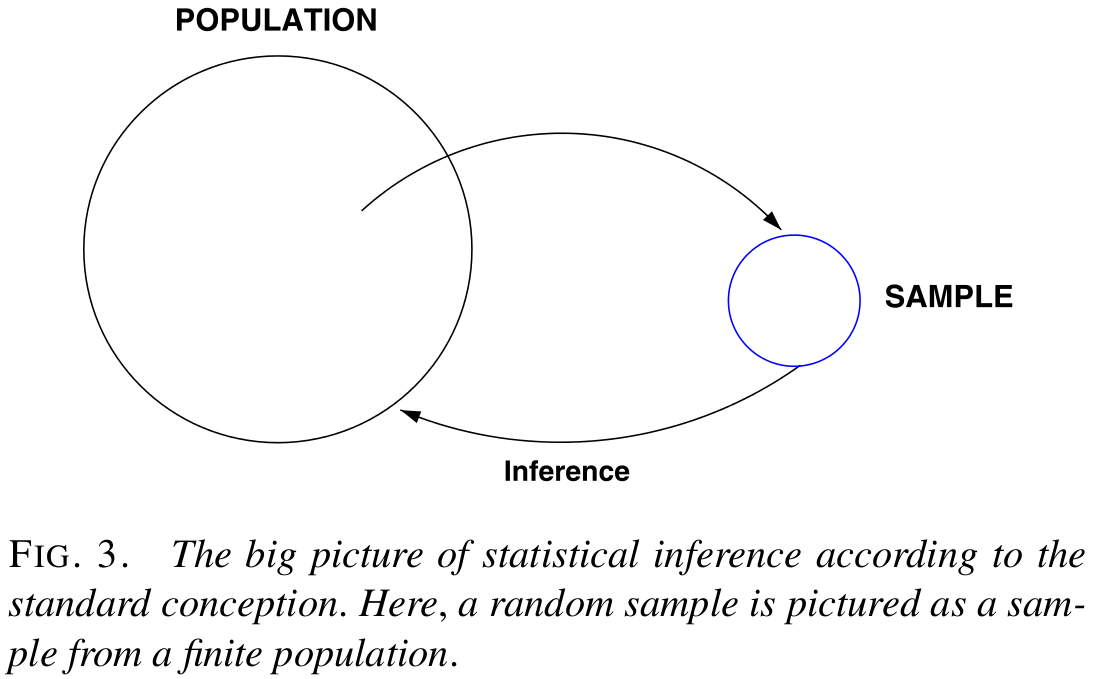
\includegraphics[width=0.8\textwidth,height=0.80\textheight,keepaspectratio=true,clip=true,trim=0 170 0 0]{kass_11_statistical-inference_fig3}%
    \end{center}
  }
  \only<3>{
    \begin{center}
      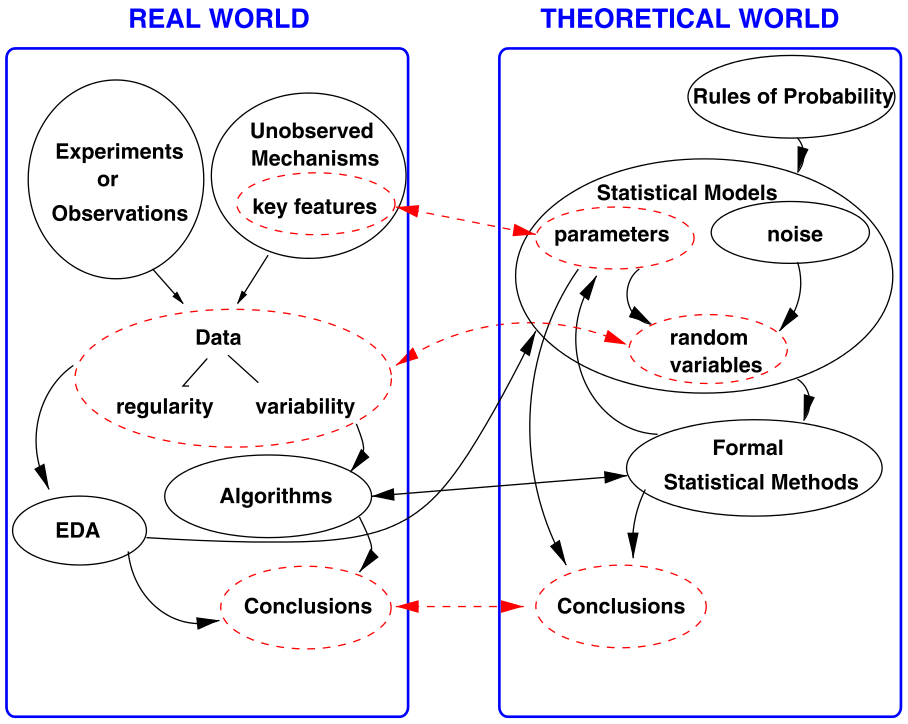
\includegraphics[width=0.8\textwidth,height=0.80\textheight,keepaspectratio=true]{kass_11_statistical-inference_fig4}%
    \end{center}
  }
\end{frame}

\begin{frame}
  \frametitle{A gloomy title, but crucial statistical advice}
  \begin{center}
    
\includegraphics[width=0.95\textwidth,height=0.90\textheight,keepaspectratio=true]{2005-08_JIoannidis_title}%
  \end{center}
  \pause
  \begin{itemize}
  \item Did you hear about \href{http://dx.doi.org/10.1371/journal.pmed.0020124}{this paper}?
  \end{itemize}
  \bigskip
  \pause
  \begin{center}
    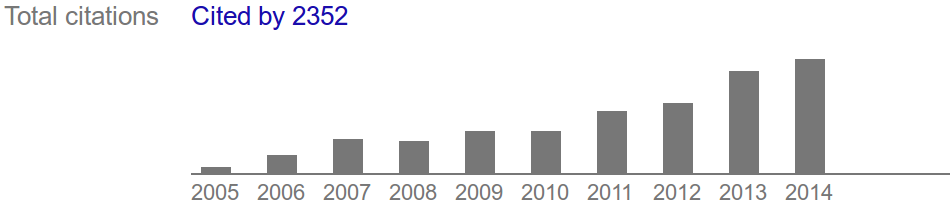
\includegraphics[width=0.95\textwidth,height=0.90\textheight,keepaspectratio=true]{2005-08_JIoannidis_citations}%
  \end{center}
  \pause
  \begin{itemize}
  \item Did you read it?
  \end{itemize}
\end{frame}

\begin{frame}
  \frametitle{Positive Predictive Value (PPV)}
  post-study probability that a significant research finding is true
  \begin{center}
    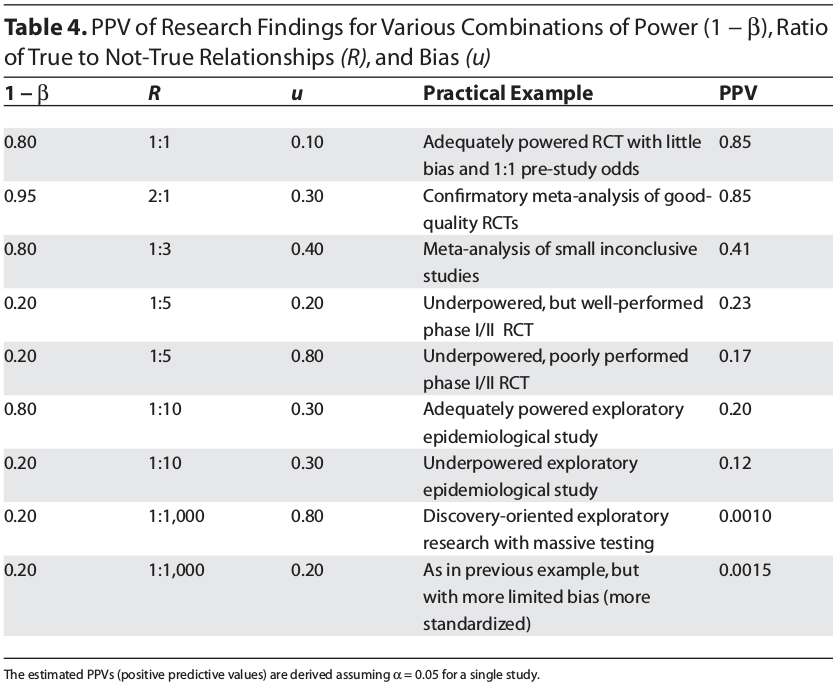
\includegraphics[width=\textwidth,height=0.7\textheight,keepaspectratio=true]{ioannidis_05_false-research-findings_tab4}%
  \end{center}
\end{frame}

\begin{frame}
  \frametitle{It's not only about weak power and high bias...}
  \begin{center}
    
\includegraphics[width=0.85\textwidth,height=0.80\textheight,keepaspectratio=true]{baggerly_09_forensic-bioinfo_title-abstract}%
  \end{center}
\end{frame}

\begin{frame}
  \frametitle{A hopeful title, and no less crucial advice}
  \begin{center}
    
\includegraphics[width=0.95\textwidth,height=0.90\textheight,keepaspectratio=true]{2014-10_JIoannidis_title}%
  \end{center}

  Read it \href{http://dx.doi.org/10.1371/journal.pmed.1001747}{here}!
  
  \bigskip
  
  \begin{center}
    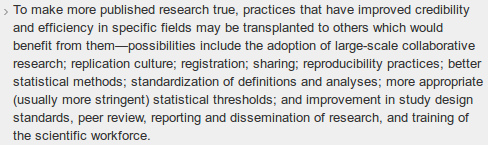
\includegraphics[width=0.95\textwidth,height=0.90\textheight,keepaspectratio=true]{2014-10_JIoannidis_summary-point}%
  \end{center}
\end{frame}

\begin{frame}
  \frametitle{Reprod. Research in Computational Science (\href{http://dx.doi.org/10.1126/science.1213847}{Peng, 2011})}
  \begin{center}
    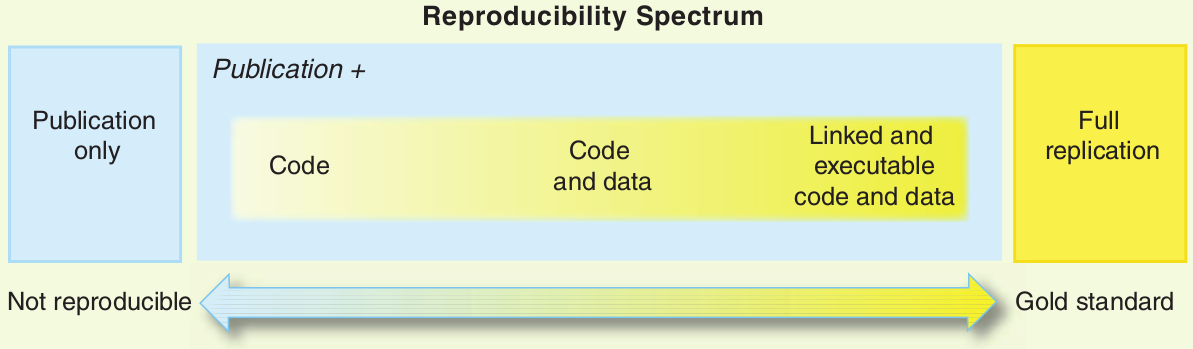
\includegraphics[width=0.95\textwidth,height=0.90\textheight,keepaspectratio=true]{peng_11_reproducible-research_fig1}%
  \end{center}
  \pause
  \begin{itemize}
  \item Are you a computational scientist?
    \pause
    \begin{itemize}
    \item Do you use Excel? R? Do you plot histograms? Do you average columns of numbers, and calculate variances?
    \end{itemize}
    \bigskip
    \pause
  \item Where are you along the spectrum?
  \end{itemize}
\end{frame}

\begin{frame}
  \frametitle{Let us start with code...}
  Claerbout \& Karrenbach (1992):
  \begin{quote}
    An article about a computational result is advertising, not scholarship. The actual scholarship is the full software environment, code and data, that produced the result.
  \end{quote}
  
  \bigskip
  \pause
  
  Buckheit \& Donohoe (1995):
  \begin{quote}
    Publishing figures or results without the complete software environment could be compared to a mathematician publishing an announcement of a mathematical theorem without giving the proof.
  \end{quote}
\end{frame}

\begin{frame}
  \frametitle{... and now data.}
  \begin{center}
    
\includegraphics[width=0.75\textwidth,height=0.90\textheight,keepaspectratio=true]{2013-06_DZamir_title}%
  \end{center}
  \pause
  \begin{quote}
    Currently, virtually none of the data generated from the hundreds of phenotypic studies conducted each year are being made publically available as raw data; thus there is little we can learn from past experience when making decisions about how to breed better crops for the future.
  \end{quote}
  
  \bigskip
  \pause
  
  Zamir (\href{http://dx.doi.org/10.1126/science.1258941}{Science, 2014}):
  \begin{center}
    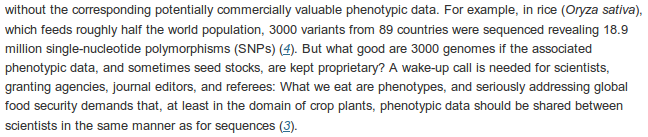
\includegraphics[width=0.95\textwidth,height=0.90\textheight,keepaspectratio=true]{2014-09_DZamir_text}%
  \end{center}
\end{frame}

\begin{frame}
  \frametitle{Incentives, to be improved}
  \begin{center}
    
\includegraphics[width=0.8\textwidth,height=0.90\textheight,keepaspectratio=true]{2014-10_Nature_code-share}%
  \end{center}
  
  \begin{center}
    
\includegraphics[width=1\textwidth,height=1.2\textheight,keepaspectratio=true]{2014-10_PLoS_data-availability}%
  \end{center}
  
  \bigskip
  \pause
  
  \href{http://prodinra.inra.fr/?locale=en}{Prod'INRA}: automatic export of productions for individual assessment, including softwares, databases, biological material, etc
\end{frame}

\begin{frame}
  \frametitle{But that's not it!}
  \small
  Blocker \& Meng (\href{http://dx.doi.org/10.3150/13-bejsp16}{Bernoulli, 2013}):
  \begin{quote}
    Decisions made in preprocessing constrain all later analyses and are typically irreversible. Hence, data analysis becomes a collaborative endeavor by all parties involved in data collection, preprocessing and curation, and downstream inference.
  \end{quote}
  \normalsize
  
  \begin{center}
    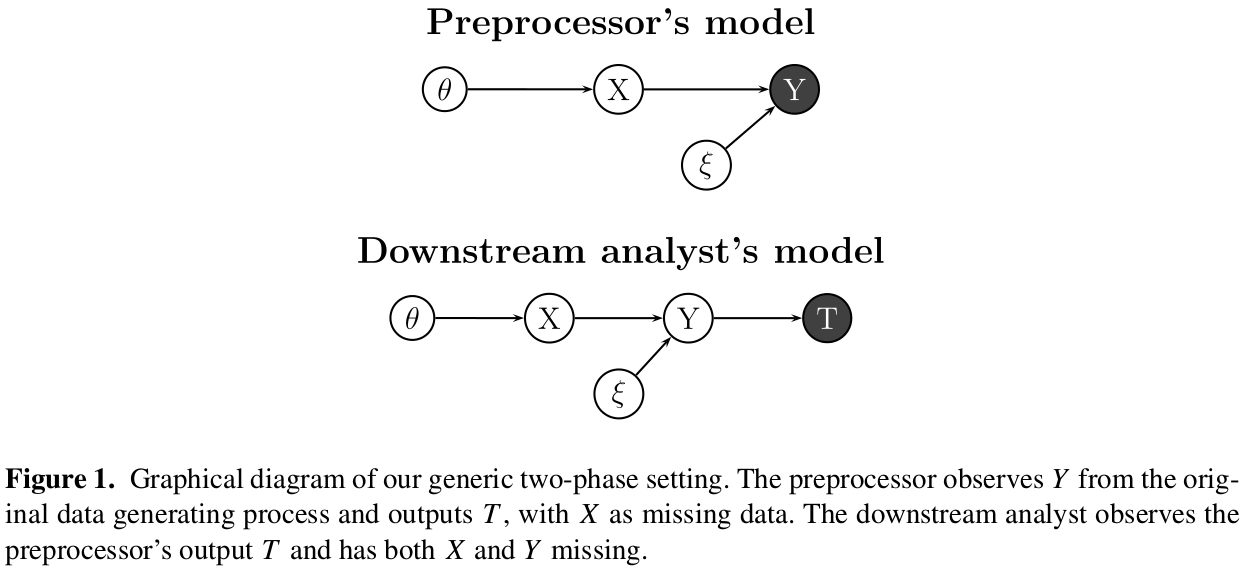
\includegraphics[width=0.95\textwidth,height=0.90\textheight,keepaspectratio=true,clip=true,trim=0 120 0 0]{blocker_13_preprocessing_fig1}%
  \end{center}
\end{frame}

\begin{frame}
  \frametitle{After all, why is reproducibility important?}
  Which reason(s) would you choose?
  \bigskip
  \pause
  \begin{itemize}
  \item reproducing work is also the first step to extending it
    \medskip
  \item we are forgetful, error-prone (or dishonest)
    \medskip
  \item helps communication with your collaborators
    \medskip
  \item bigger visibility in the community
    \medskip
  \item we are mostly funded by public money
    \medskip
  \item ...
  \end{itemize}
\end{frame}

\section{Spectrum of solutions}

\begin{frame}
  \frametitle{Multi-dimensional space of "projects"}
  \begin{itemize}
  \item \alert{question}: mono- or inter-disciplinary; closer to applied or to basic research
    \begin{itemize}
    \item won't be discussed here, but obviously crucial...
    \end{itemize}
    \medskip
    \pause
  \item \alert{data}: few small files or many large files; custom or standardized formats; databases
    \medskip
    \pause
  \item \alert{code}: in interpreted languages (e.g. R, Python, Perl, Bash) or compiled languages (e.g. C, C++, Fortran)
    \medskip
    \pause
  \item \alert{model}: informal (any word processor is enough, e.g. Writer, Word) or formal (many equations, much easier in LaTeX)
    \medskip
    \pause
  \item \alert{collaborators}: professional scientist or anyone else; beginner or experienced; "open curious" or already fully proficient
  \end{itemize}
\end{frame}

\begin{frame}
  \frametitle{Initial steps toward reproducible research}
  Karl Broman's tutorial: \url{http://kbroman.org/steps2rr/}
  
  \bigskip
  
  \begin{enumerate}
  \item Everything with a script
  \item Organize your data and code
  \item Automate the process
  \item Turn scripts into reproducible reports
  \item Turn repeated code into functions
  \item Package functions for reuse
  \item Use version control
  \end{enumerate}
  
  \bigskip
  \pause
  
  See also: \url{http://software-carpentry.org/}
\end{frame}

\begin{frame}[fragile]
  \frametitle{A text editor, not a word processor}
  \begin{itemize}
  \item word processors: \href{https://www.libreoffice.org/discover/writer/}{LibreOffice Writer}, Microsoft Word, etc
  \item text editors: \href{https://www.gnu.org/software/emacs/}{Emacs}, Vim, \href{https://notepad-plus-plus.org/}{Notepad}++, \href{https://wiki.gnome.org/Apps/Gedit}{Gedit}, Geany, etc
  \end{itemize}
  
  \bigskip
  \pause
  
  Why \alert{knowing/mastering a good text editor is crucial}?
  \begin{itemize}
  \item essential tool of any data analysis, e.g. scripts
  \item light-weight markup languages convert plain text to PDF/HTML/odt/docx/etc, check out \href{http://johnmacfarlane.net/pandoc/}{pandoc}
  \item delivers full power of \href{http://www.ibm.com/developerworks/aix/library/au-unixtext/index.html}{text manipulation tools}, e.g. \verb+diff+ to compare, \verb+grep+ to search, \verb+awk+ to extract, ...
  \item allows efficient use of version control systems such as \href{http://www.git-scm.com/}{git}
  \end{itemize}
\end{frame}

\begin{frame}[fragile]
  \frametitle{Project organization}
  Follow the spirit of Noble (\href{http://dx.doi.org/10.1371/journal.pcbi.1000424}{PLoS Comput Biol, 2009}):
  \begin{itemize}
  \item someone unfamiliar with your project should be able to look at your computer files and understand in detail what you did and why;
  \item everything you do, you will probably have to do it over again.
  \end{itemize}
  
  \bigskip
  \pause
  
  \begin{enumerate}
  \item choose a short project name and create a directory
  \item give brief explanations in a text file named README
  \item describe sharing/modifying rights in a text file named COPYING or LICENSE
  \item list authors in a text file named AUTHORS
  \item create subdirectories \verb+doc/+, \verb+data/+, \verb+src/+ and \verb+results/+
  \end{enumerate}
\end{frame}

\begin{frame}
  \frametitle{Version control systems (VCS)}
  Karl Broman on VCS:
  \begin{itemize}
  \item not strictly necessary for \emph{reproducibility}, but can be hugely useful for \emph{sanity}
  \item requires a big initial investment in time and effort, but become a natural part of your daily workflow after a month or so
  \item huge \emph{short-term} advantages in collaborative projects (keeping in sync, merging simultaneous changes)
  \end{itemize}
  
  \bigskip
  \pause
  
  My advice: use \alert{git} (free software; multi-platform; used all over the globe by programmers, scientists, journalists, etc)
  \begin{itemize}
  \item download it from \url{http://git-scm.com/}
  \item \emph{read} chapters 1 to 3 of the official \href{http://git-scm.com/book/en/v2}{book}
  \end{itemize}
\end{frame}

\begin{frame}[fragile]
  \frametitle{Two examples}
  \begin{enumerate}
  \item \alert{project "ligth"}: a few small data files; laptop; classical models; available implementations for interpreted languages
    \begin{itemize}
    \item ok to re-run the whole analysis from time to time
    \item write notebook in text file in \href{http://cran.r-project.org/web/packages/rmarkdown/index.html}{Rmd} format and use \href{http://www.rstudio.com/products/rstudio/download/}{RStudio}
    \end{itemize}
    \bigskip
    \pause
  \item \alert{project "heavy"}: many large files, e.g. sequencing data; cluster; possibly new models and implementations
    \begin{itemize}
    \item can't re-run the whole analysis because of intensive computations
    \item write notebook in text file in \href{http://orgmode.org/}{org} format and use \href{https://www.gnu.org/software/emacs/}{Emacs} or \href{http://johnmacfarlane.net/pandoc/}{pandoc}
    \end{itemize}
  \end{enumerate}
\end{frame}

\begin{frame}[fragile]
  \frametitle{Project "light"}
  \begin{enumerate}
  \item create your project directory: \verb+README+, \verb+COPYING+, \verb+AUTHORS+, \verb+doc/+, \verb+data/+, \verb+src/+, \verb+results/+
  \item (re-)install the latest version of RStudio: \url{http://www.rstudio.com/}
  \item visit \href{https://github.com/timflutre/tuto-reproducible-research}{github.com/timflutre/tuto-reproducible-research} and download the Rmd file in \verb+project_light/+
  \item convert it from Rmd to HTML in RStudio by clicking on \verb+Knit to HTML+
  \end{enumerate}
  \bigskip
  \pause
  Play!
  \small
  \url{https://github.com/csgillespie/statslang/tree/master/R}
  \url{http://cran.r-project.org/web/packages/agridat/index.html}
  \url{http://cran.r-project.org/web/packages/HistData/}
\end{frame}

\begin{frame}[fragile]
  \frametitle{Project "heavy"}
  Usually, if large data, then computer cluster, and "shared space":
  \begin{itemize}
  \item \verb+external_public/+, \verb+external_private/+, \verb+internal/+
  \end{itemize}
  
  \bigskip
  \pause
  
  \begin{enumerate}
  \item create the backbone for \verb+project_heavy+ in your home
  \item version it with git, and push it to the server
  \item clone the repository for \verb+project_heavy+ in the shared space
  \item put the large data files \verb+data/+ in the shared space, but don't version them
  \item edit versioned files in your home, and commit/push
  \item run intensive computations in the shared space (coordinate with other users!)
  \item update (\verb+pull+) repository on the shared space (need one \verb+origin-<user>+ per user)
  \end{enumerate}
\end{frame}

\begin{frame}
  \frametitle{Are you teaching?}
  Example in \alert{statistics} from Matthew Stephens: class notes versioned with git and hosted \href{https://github.com/stephens999/stat302}{on GitHub}
  
  \bigskip
  
  \begin{center}
    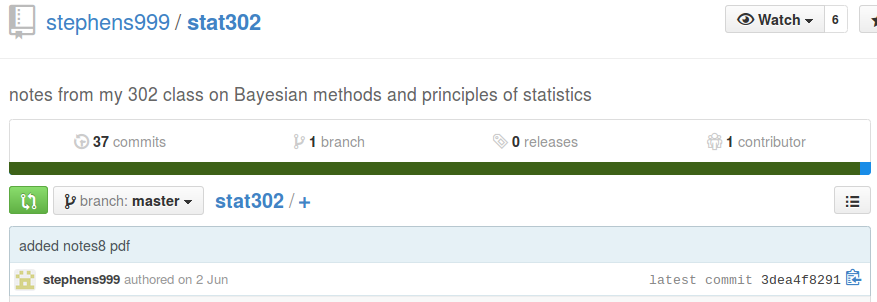
\includegraphics[width=\textwidth,height=\textheight,keepaspectratio=true]{mstephens_stat302}%
  \end{center}
\end{frame}  

\begin{frame}
  \frametitle{Are you teaching? Cont'd}
  Example in \alert{population genetics} from Graham Coop: class notes versioned with git and hosted \href{https://github.com/cooplab/popgen-notes}{on GitHub}
  
  \bigskip
  
  \begin{center}
    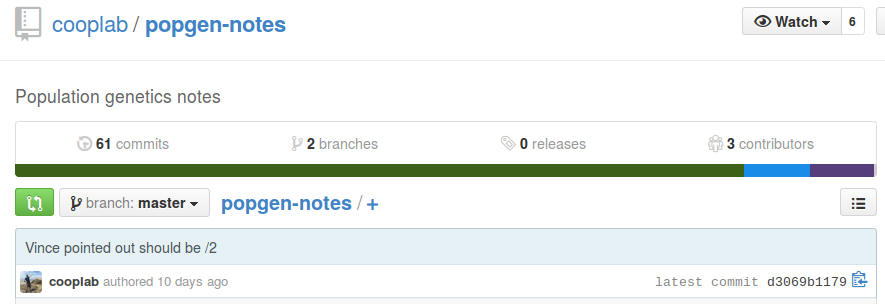
\includegraphics[width=\textwidth,height=\textheight,keepaspectratio=true]{cooplab_popgen}%
  \end{center}
\end{frame}  

\begin{frame}
  \frametitle{Are you writing an article?}
  Example in \alert{plant biology} from Rubén Rellán Álvarez: article (text, figures) and software versioned with git and hosted \href{https://github.com/rr-lab/glo_roots}{on GitHub}
  
  \bigskip
  
  \begin{center}
    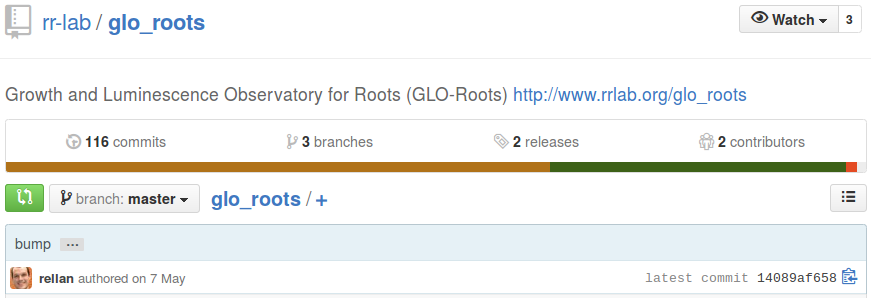
\includegraphics[width=\textwidth,height=\textheight,keepaspectratio=true]{rrlab_roots}%
  \end{center}
\end{frame}

\begin{frame}
  \frametitle{Are you writing a book?}
  Example in \alert{mathematics} from the "Homotopy Type Theory" group which started at Princeton (IAS) and now writes a book versioned with git and hosted \href{https://github.com/HoTT/book}{on GitHub}
  
  \bigskip
  
  \begin{center}
    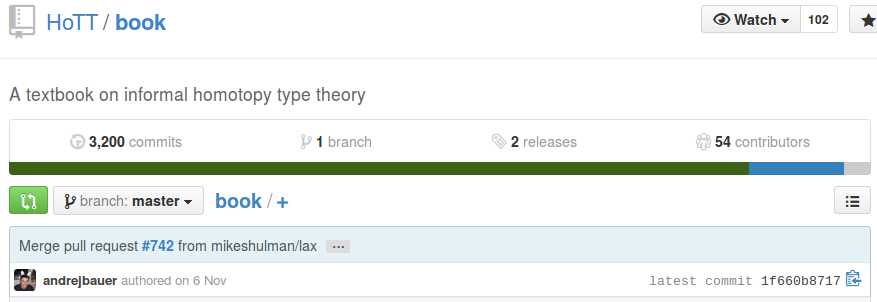
\includegraphics[width=\textwidth,height=\textheight,keepaspectratio=true]{HoTT_book}%
  \end{center}
\end{frame}

\begin{frame}
  \frametitle{Take-home message}
  Whatever the exact tools you are using, it is the spirit that is important!
  
  \bigskip
  \pause
  
  \begin{itemize}
  \item How well does your behavior favor others understanding and building on your work?
    \bigskip
  \item When and how will you start?
  \end{itemize}
\end{frame}

\end{document}
